This exercise has been completed in the attached \textit{PCA and classification.ipynb} Jupyter Notebook. The most relevant bits of source code can be seen here as well, though all comments are left out. It should be noted that the pca function is based on the one from lecture slides, but it has been modified. The full source code is in the notebook, along with comments:
\begin{verbatim}
def pca(data):
    d, N = data.shape

    center = np.mean(data, 1)
    centers = np.matlib.repmat(center, N, 1)
    data_cent = data - np.transpose(centers)
    
    Sigma = np.cov(data_cent)
    evals, evecs = np.linalg.eigh(Sigma)
    
    return np.flip(evals,0), np.flip(evecs, 1), data_cent

eVals, eVecs, data_cent = pca(trainset.T)

PC1 = eVecs[:,0]
PC2 = eVecs[:,1]

PC1projs = np.matmul(data_cent.T,PC1)
PC2projs = np.matmul(data_cent.T,PC2)
\end{verbatim}
The resulting plot can be seen here:\\
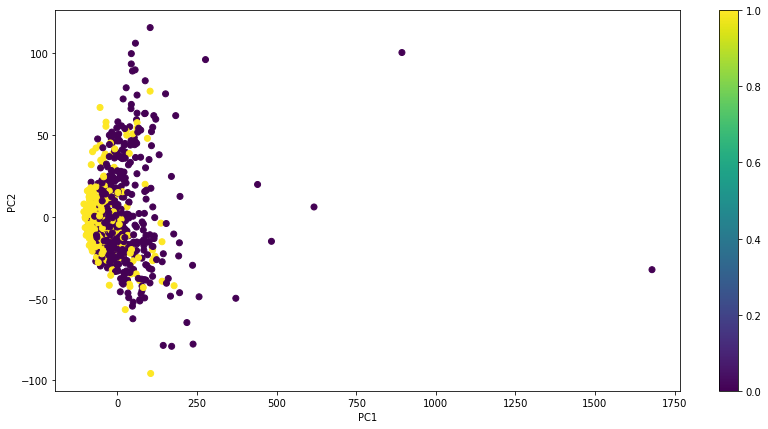
\includegraphics[width=\linewidth]{5a1.png}
We can see here that the two different labels can be quite difficult to differentiate, as they are very close together based on these two pricipal components. We do however, see that the label '0' has slightly higher variance in its clustering.